\documentclass[10pt,a4paper]{article}
\usepackage[T1]{fontenc}
\usepackage[a4paper]{geometry}
\usepackage{xcolor}
\usepackage{amssymb}
\usepackage{amsmath}
\usepackage{graphicx}
\usepackage{tabularx}
\usepackage{multirow}
\usepackage{subfigure}
\usepackage{verbatim}
\usepackage{fancyhdr}
\usepackage{listings}
\usepackage{../common/espacs}

%\input{../common/commands.tex}

\newcommand*{\vect}[1]{\boldsymbol{#1}}
\newcommand*{\mat}[1]{\boldsymbol{#1}}

\title{Exercise Session 5}
\date{November 9, 2012}

\pagestyle{fancy}
\headheight 35pt

\begin{document}
\lstset{language=[ISO]C++}
\maketitle

\section*{Data mining: $k$-means clustering}

$k$-means clustering is a common method used in data mining, which aims to
partition $N$ objects into $k$ clusters, with $k << N$. The clusters are built
such as each object belongs to the \emph{nearest} cluster, so there must be a
notion of distance between objects.

An object example can be a point in $\RR^n$ equipped with the Euclidean norm. In
this case the distance would be computed with respect to the centroid of the
cluster and the space would be partitioned in Voronoi cells. The approach is
however more genaral, it can be applied to any set of objcts with a kwnoledge of
a distance between then, e.g. functions in a suitable space and a suitable norm,
etc.

%%%%%%%%%%%%%%
\begin{figure}[htb]
\centering
$\vcenter{\hbox{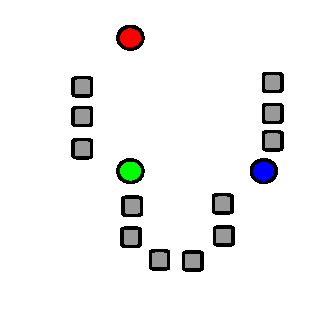
\includegraphics[width=.3\textwidth]{fig/wiki1}}}$
\hfil
$\vcenter{\hbox{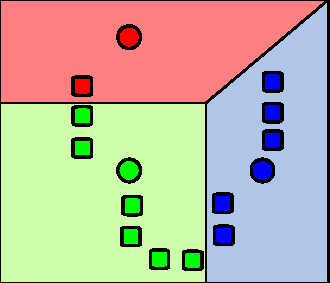
\includegraphics[width=.3\textwidth]{fig/wiki2}}}$
\\[1ex]
$\vcenter{\hbox{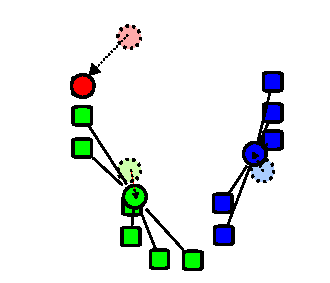
\includegraphics[width=.3\textwidth]{fig/wiki3}}}$
\hfil
$\vcenter{\hbox{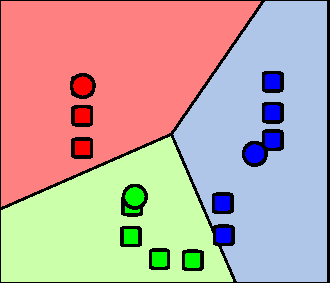
\includegraphics[width=.3\textwidth]{fig/wiki4}}}$
\caption{$k$-means algorithm in $\RR^2$. The squares represent the objects to be
clustered, while the circles represent the centroids of the partitions. Each
}
\label{fig:alg}
\end{figure}
%%%%%%%%%%%%%%
The problem is NP-hard, but an algorithm can be devised in order to approach a
local optimum. The algorithm is depicted in Fig. \ref{fig:alg} for the case of
points in $\RR^2$. Given a set of initial centroids, the objects are associated
to the nearest centroid to build up the clusters. Afterwords, the centroid is
updated to the point that minimizes the distance between the objects that belong
to the partition. In the case of the Euclidean norm it will be the barycenter of
the points in the cluster. This concludes a step of the algorithm, that is
repeated starting again assigning the points to the nearest centroid.

The algorithm stops when the clusters are fixed: when all the points are again
assigned to the same partition, the update of the centroids gives a null
increment. Note that, since we only reach a local optimum, the solution is
dependent on the choice of the initial guess for the centroids.

\section*{Exercise}

Starting from the solution of a previous exercise session on iterative methods
to compute a zero of a function

\begin{enumerate}

  \item Templetize the methods so that they can be used with different 
  floating point number formats.
  
  \item Implement a template functor that manages the function and optionally
  the derivative of the function to be used by the method. Analyze all the
  possible implementation strategy with their advantages and drawbacks. Take
  care in converting also the \cpp{apply} method to a template one.

%  \item () Add a template parameter to the whole class hierarchy. The template is
%  introduced to allow the use of a function or a functor. Also in this case the
%  implementation details can vary, with advantages and drawbacks.

  \item (optional) Substitute the dynamic polymorphism paradigm with a static polymorphism
  paradigm.
\begin{lstlisting}
// dynamic polymorphism
class Base
{
  virtual void foo() {}
};

class Derived: public Base
{
  void foo() {}
};

// static polymorphism
template <typename DerivedT>
class Base
{
  void foo() { static_cast<DerivedT *>(this)->foo(); }
}

class Derived: public Base<Derived>
{
  void foo() {}
};

\end{lstlisting}

\end{enumerate}



\section*{Solution}

\begin{enumerate}

\item Main aspects of the solution for question 1:

\begin{itemize}

\item Both declarations and definitions of templated classes and methods mus be in a header files, for this reason we collected all the class declarations and implementations in one single header file. Other code organizations are possible as explained in the lectures.

\item In a class template derived names are 
resolved only when a template class is instantiated 
so methods and attributes in the derived classes {\tt Bisection}, {\tt Newton}, and {\tt Robust} that are inherited from the base class {\tt IterativeMethod}
must be prepended by {\tt this->} so that the compiler
can understand they are dependent identifiers and only try to resolve them when the templated classes are instantiated.

\item For a similar reason the typedefs in the base
class need to be fully qualified when used in the derived classes.

\item Using the {\tt STL} class template {\tt numeric\_limits}.

\end{itemize}

Main file:

\lstinputlisting{ex8_sol1/bn.cpp}

Header defining all the class templates:
\lstinputlisting{ex8_sol1/iterativeMethod.hpp}

\item Main aspects of the solution for question 2:

\begin{itemize}
\item Notice that, unless specifying {\tt -std=c++11}, a space is required when two {\tt >} 
symbols appear consecutively in a template parameter list.
\end{itemize}

Main file:

\lstinputlisting{ex8_sol2/bn.cpp}

Header defining all the class templates:
\lstinputlisting{ex8_sol2/iterativeMethod.hpp}

\end{enumerate}






\end{document}
